
\resetcounters
\bibliographystyle{asp2010}

\markboth{Schaaff et al.}{Feedback About Application Developments}

\title{Feedback About Astronomical Application Developments for Mobile Devices}
\author{A.~Schaaff,$^1$ T.~Boch,$^2$, P.~Fernique,$^2$ R.~Houpin,$^4$ V.~Kaestl\'e,$^3$ M.~Royer,$^4$ J.~Scheffmann,$^4$ and A.~Weiler$^4$
\affil{$^1$CDS, CNRS, Observatoire astronomique, 11 rue de l'Universit\'e 67000 Strasbourg}
\affil{$^2$CDS, UDS,  Observatoire astronomique, 11 rue de l'Universit\'e 67000 Strasbourg}
\affil{$^3$Universit\'e de Strasbourg,  67000 Strasbourg}
\affil{$^4$Universit\'e de Lorraine, 54000 Nancy}}

\aindex{Schaaff, A.}
\aindex{Boch, T.}
\aindex{Fernique, P.}
\aindex{Houpin, R.}
\aindex{Kaestl\'e, V.}
\aindex{Royer, M.}
\aindex{Scheffmann, J.}
\aindex{Weiler, A.}

\begin{abstract}
Within a few years, Smartphones have become the standard for mobile telephony, and we are now witnessing a rapid development of Internet tablets. These mobile devices have enough powerful hardware features to run more and more complex applications. In the field of astronomy it is not only possible to use these tools to \ssindex{data!access}access data via a simple browser, but also to develop native applications reusing libraries (\ssindex{computer languages!Java}Java for \ssindex{computing!mobile!Android}Android, \ssindex{computer languages!Objective-C}Objective-C for \ssindex{computing!mobile!iOS}iOS) developed for desktops. We have been working for two years on mobile application development and we now have the skills in native \ssindex{computing!mobile!iOS}iOS and \ssindex{computing!mobile!Android}Android development, Web development (especially HTML5, \ssindex{computer languages!JavaScript}JavaScript, CSS3) and conversion tools (PhoneGap) from Web development to native applications. The biggest change comes from human/computer interaction that is radically changed by the use of multitouch. This interaction requires a redesign of interfaces to take advantage of new features (simultaneous selections in different parts of the screen, etc.). In the case of native applications, the distribution is usually done through online stores (App Store, Google Play, etc.) which gives visibility to a wider audience. Our approach is not only to perform testing of materials and developing of prototypes, but also operational applications. The native application development is costly in development time, but the possibilities are broader because it is possible to use native hardware such as the gyroscope and the accelerometer, to point out an object in the sky. Development depends on the Web browser and the rendering and performance are often very different between different browsers. It is also possible to convert Web developments to native applications, but currently it is better to restrict this possibility to light applications in terms of functionality. Developments in HTML5 are promising but are far behind those available on desktops. HTML5 has the advantage of allowing development independent from the evolution of the mobile platforms ("write once, run everywhere"). The upcoming Windows 8 support on desktops and Internet tablets as well as a mobile version for smartphones will further expand the native systems family. This will enhance the interest of Web development.
\end{abstract}

\section{Introduction}
In 2010, we started development for \ssindex{computing!mobile!Android}Android with a prototype based on \ssindex{catalogs!services!VizieR}VizieR Mine. In 2011 we developed SkySurveys, which \ssindex{software!reuse}reuses \ssindex{libraries!HEALPix}HEALPix \ssindex{computer languages!Java}Java libraries from \ssindex{applications!Aladin}Aladin. It lets you navigate through surveys. It also uses the \ssindex{libraries!OpenGL}\ssindex{software!tools!OpenGL}OpenGL library. In 2012 we developed SkyObjects natively for \ssindex{computing!mobile!iOS}iOS and \ssindex{computing!mobile!Android}Android. This application provides information about astronomical objects, stores them locally with the user's own information and points out the objects in the sky, etc. We also tested the same type of application with HTML5 and we are working to improve its display performance. SkyObjects is in the deposit process for Google Play and the App Store. SkySurveys is available directly from the\ssindex{Centre de Donn\'ees astronomiques de Strasbourg (CDS)} CDS Web pages. We will present these developments with a critical eye.\ooindex{Aladin, ascl:1112.019} 

\section{Different Ways of Development}

We have explored three ways to build applications for mobile devices.
It is possible to develop Web applications in HTML4/5 as for desktops, but with dedicated \ssindex{computer languages!JavaScript}Javascript libraries like Mobile \ssindex{computing!mobile!framework!jQuery}\ssindex{libraries!jQuery}jQuery which are optimized for mobile devices. A second solution is to develop a native application in \ssindex{computer languages!Java}Java for \ssindex{computing!mobile!Android}Android, \ssindex{computer languages!Objective-C}Objective C for \ssindex{computing!mobile!iOS}iOS, etc. 
A third solution is to develop Web applications in HTML and \ssindex{computer languages!JavaScript}javascript and to convert these\ssindex{web!applications} applications to pseudo native applications through converters like PhoneGap. We have not tried any another way which consists of the development in one language (for example \ssindex{computer languages!Java}Java) and the conversion to an another like \ssindex{computer languages!Objective-C}Objective-C. It is possible to find a few frameworks to do it like J2ObjC which converts just the \ssindex{computer languages!Java}Java code (data \ssindex{data!access}access, etc.) excepting the \ssindex{software!user interfaces}GUI side.

\subsection{Web Development}
Web development is the fastest way to develop an application on mobile devices. A number of frameworks and \ssindex{computer languages!JavaScript}javascript libraries are now available and it is possible to create a very nice application in a few hours or at least in a few days for a well designed application. A mobile version of the\ssindex{Centre de Donn\'ees astronomiques de Strasbourg (CDS)} CDS Portal has been developed this way (see Fig.~\ref{O28:1}).

\begin{figure}[ht] \center
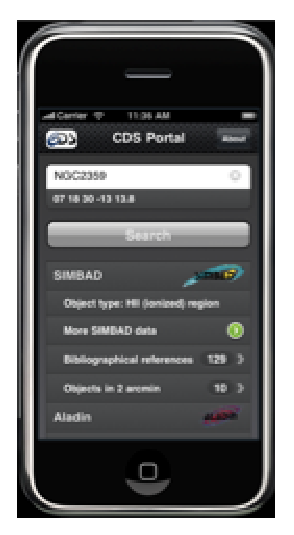
\includegraphics[scale=0.7]{part5/Schaaff_O28/O28_f4.eps}
\caption{CDS mobile portal} 
\label{O28:1}
\end{figure}

\subsection{Native Development}
The number of \ssindex{libraries!HEALPix}HEALpix \citep{gorski_2005} available\ooindex{HEALPix, ascl:1107.018} surveys is growing and a few \ssindex{libraries!HEALPix}HEALPix visualizers are available, like \ssindex{applications!Aladin}Aladin through the Allsky mode \citep{fernique_2010}. This mode runs well on a desktop or a laptop with good performance but it was a real challenge to develop a visualizer for smartphones and Internet tablets. We decided to develop it on \ssindex{computing!mobile!Android}Android because it was possible to \ssindex{software!reuse}reuse a part of the \ssindex{applications!Aladin}Aladin source written in \ssindex{computer languages!Java}Java. The first tests were not really good due to the basic hardware capabilities compared to a desktop. \ssindex{applications!Aladin}Aladin does not use \ssindex{libraries!OpenGL}\ssindex{software!tools!OpenGL}OpenGL but this graphical library is available on almost all the mobile devices. The new prototype implementing this library was between thirty and forty times faster and the FPS (frames per second) were sufficient to provide a fluid display. All the surveys available, and added in the future, in \ssindex{applications!Aladin}Aladin will also be available in the application called SkySurveys (see Fig.~\ref{O28:2}). It is possible to try it by downloading from the\ssindex{Centre de Donn\'ees astronomiques de Strasbourg (CDS)} CDS developer's corner. We consider this application as an advanced prototype for \ssindex{computing!mobile!Android}Android devices and we will probably not develop it the same way for \ssindex{computing!mobile!iOS}iOS devices.

\begin{figure}[ht] \center
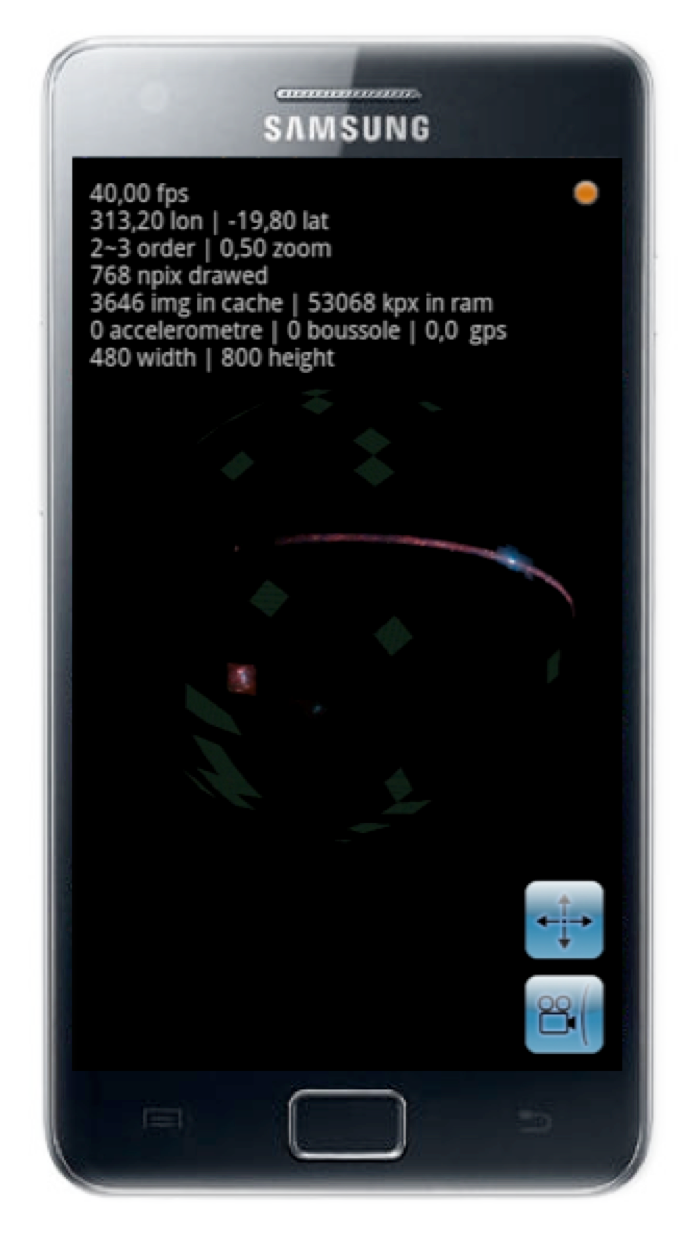
\includegraphics[scale=0.28]{part5/Schaaff_O28/O28_f1.eps}
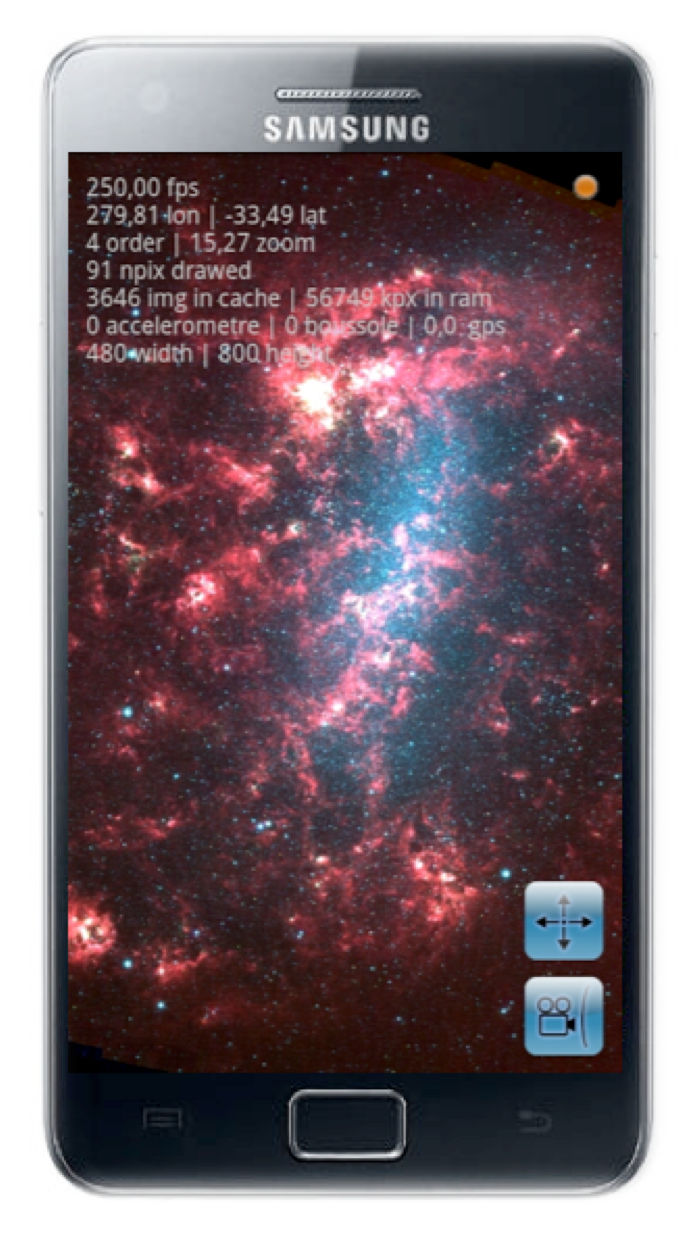
\includegraphics[scale=0.28]{part5/Schaaff_O28/O28_f2.eps}
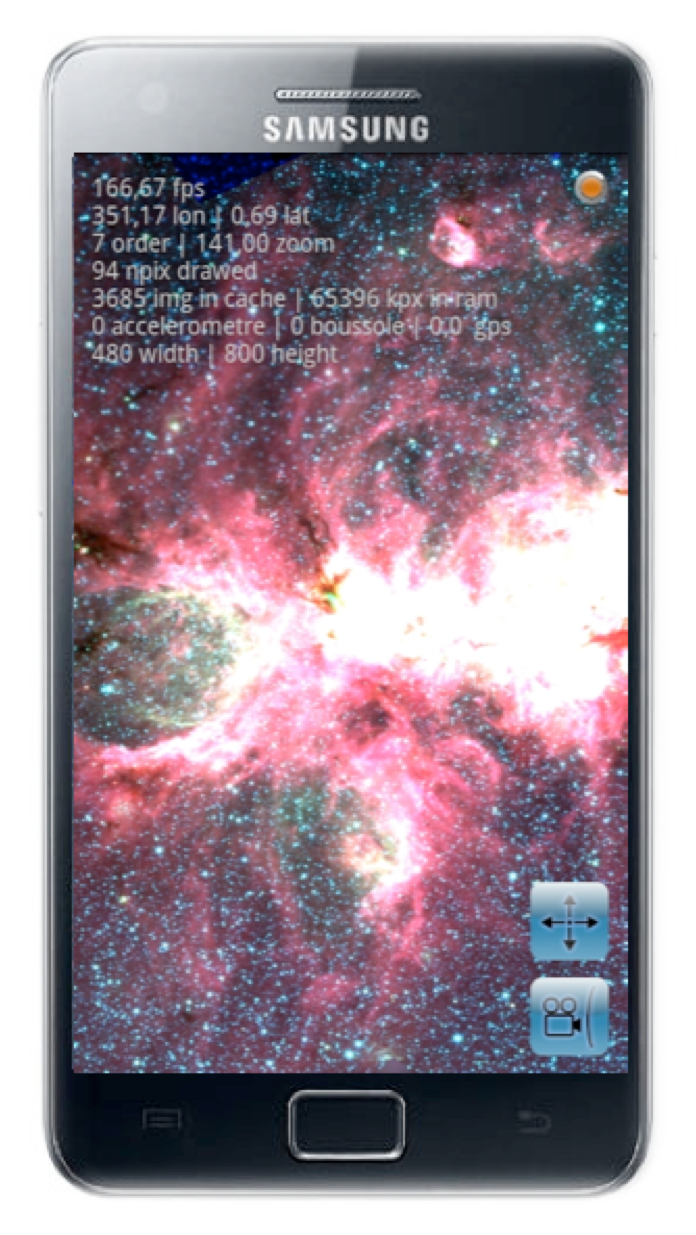
\includegraphics[scale=0.28]{part5/Schaaff_O28/O28_f3.eps}
\caption{Spitzer survey (credits JPL/NASA)} 
\label{O28:2}
\end{figure}

\subsection{Converters}
We have developed the main features of SkyObjects in HTML5 and we have converted it using PhoneGap to \ssindex{computing!mobile!iOS}iOS and \ssindex{computing!mobile!Android}Android applications. But we had a big "gap" between the final application and what we had developed directly in \ssindex{computer languages!Java}Java or \ssindex{computer languages!Objective-C}Objective-C: the generated application is not a real native application, it is just an \ssindex{computing!mobile!Android}Android or \ssindex{computing!mobile!iOS}iOS\ssindex{web!applications} application implementing an HTML5 emulator with the HTML5 Web\ssindex{web!applications} application code. So it is not a real conversion to a native language. It means also that it is not possible to convert in a native language and to modify this code. Another difficulty was also the lack of some functionalities of the mobile devices like the gyroscope  (see Fig.~\ref{O28:3}).

\begin{figure}[ht] \center
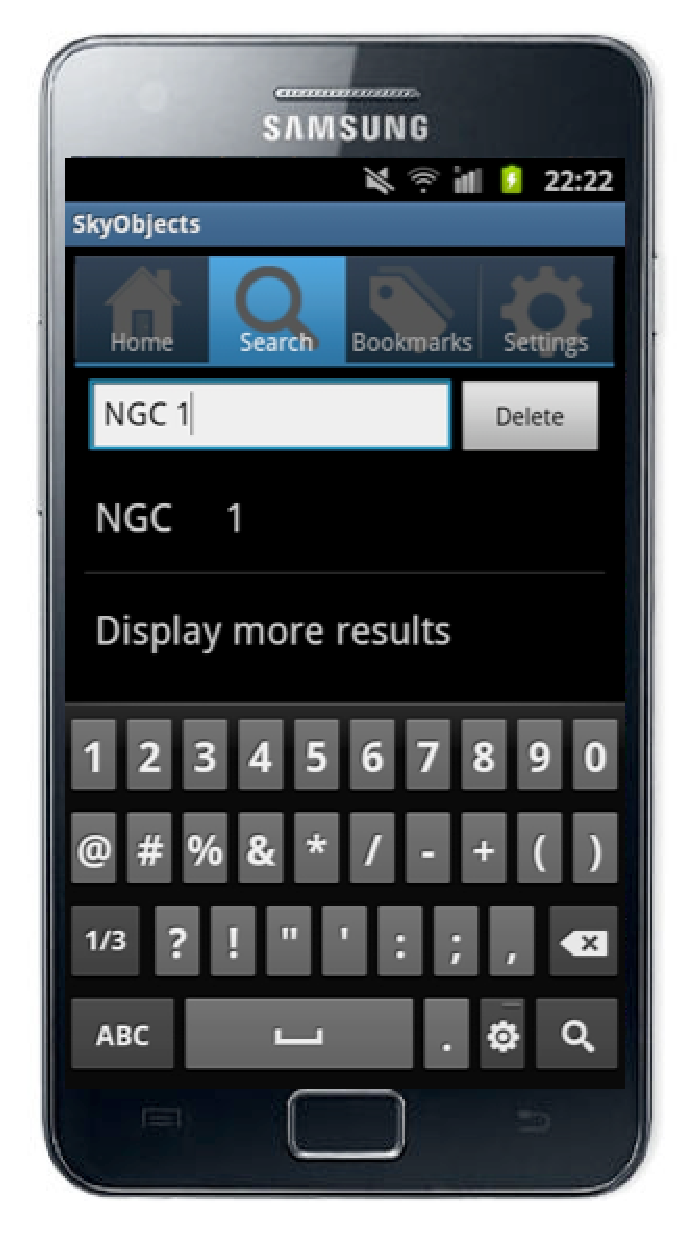
\includegraphics[scale=0.28]{part5/Schaaff_O28/O28_f5.eps}
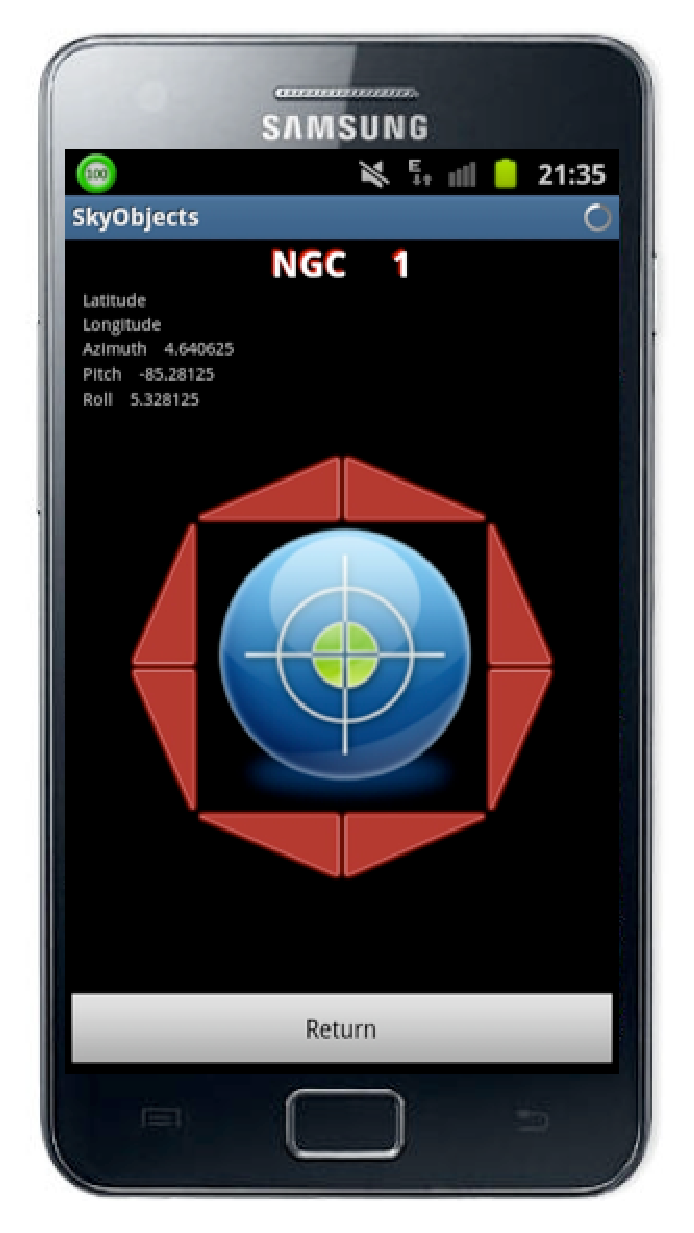
\includegraphics[scale=0.28]{part5/Schaaff_O28/O28_f6.eps}
\caption{SkySurveys with pointing functionality using the gyroscope.} 
\label{O28:3}
\end{figure}

\section{Perspectives}
We are now focusing the new developments on Web apps based on HTML5 (\url{http://www.w3.org/TR/html5/}), which can provide rich content and which should become a standard probably in about one year. As it is not easy to have both \ssindex{computer languages!Java}Java and \ssindex{computer languages!Objective-C}Objective-C skills in a team and to have enough time for native development, it has the advantage of allowing development independent of the mobile platform and to avoid the deep tests which are needed, for example on \ssindex{computing!mobile!Android}Android devices. But frameworks should also evolve and it should be easier in the future to develop applications for the main mobile operating systems without doing the work two or three times. All the experiments are detailed at \url{cds.u-strasbg.fr/resources/doku.php?id=mobiledev}.

\section{Conclusion}
The first prototypes were important to evaluate the time necessary to develop tools for mobile devices and to have a reflection about which service or application would be useful on these kinds of devices. The development of native applications for mobile devices has a high cost in terms of man power and time. It is easy to use, for example, existing \ssindex{computer languages!Java}Java \ssindex{software!source code}source code with a quick development of an \ssindex{computing!mobile!Android}Android user interface but development from scratch needs time similar to development for desktops or laptops. We think that the development of a native "app" for \ssindex{computing!mobile!Android}Android or \ssindex{computing!mobile!iOS}iOS are justified if it is not possible to provide or adapt a simple Web\ssindex{web!applications} application (HTML and \ssindex{computer languages!JavaScript}Javascript) independent from the device.

\bibliography{editor}
